\documentclass[border=10pt]{standalone}
\usepackage{pgfplots}
\pgfplotsset{compat=1.18}
\usepgfplotslibrary{fillbetween}
\begin{document}
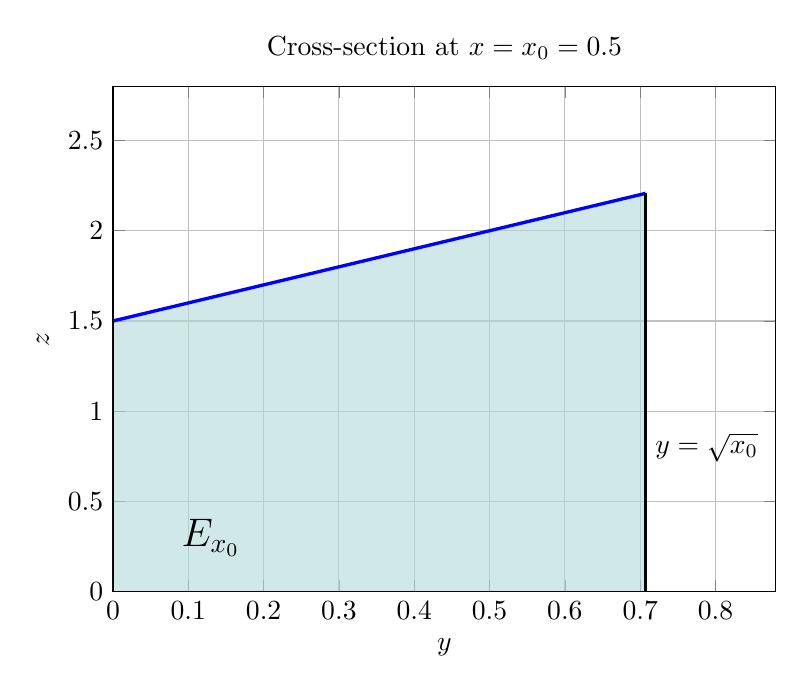
\begin{tikzpicture}
\begin{axis}[
    width=10cm, height=8cm,
    xlabel={$y$}, ylabel={$z$},
    xmin=0,xmax=0.88,ymin=0,ymax=2.8,
    title={Cross-section at $x=x_0=0.5$},
    grid=both,
    samples=200,
]
\addplot[name path=top, domain=0:0.7071, blue, very thick] {1.5+x};
\addplot[name path=bottom, domain=0:0.7071, black, thick] {0};
\addplot[teal!30, opacity=0.6] fill between[of=top and bottom];
\addplot[black, thick] coordinates {(0,0) (0,1.5)};
\addplot[black, thick] coordinates {(0.7071,0) (0.7071,2.2071)};
\node at (axis cs:0.13,0.3) {\Large $E_{x_0}$};
\node[right] at (axis cs:0.7071,0.8) {$y=\sqrt{x_0}$};
\node[below] at (axis cs:0.35,0) {$z=0$};
\end{axis}
\end{tikzpicture}
\end{document}
